\documentclass[12pt]{book}

\usepackage{stylepackage}
\theoremstyle{plain}

\begin{document}
%            %
% CHAPITRE 1 %
%            %
\setcounter{chapter}{1}
\chapter{\textmd{\textsc{\Large{Chapitre 1}}} \\ \textsl{Espaces vectoriels}}

\vfill

% INTRODUCTION
\indent{L'algèbre linéaire est l'étude des applications linéaires sur des espaces vectoriels de dimension finie. Nous apprendrons plus tard ce que signifient ces termes. Dans ce chapitre, nous allons définir les espaces vectoriels et aborder leurs propriétés élémentaires.}

\indent{Dans certains domaines des mathématiques, y compris l'algèbre linéaire, on obtient des théorèmes plus intéressants et une meilleure compréhension du sujet si l'on prend en compte les nombres complexes en même temps que les nombres réels. C'est pourquoi nous allons commencer par introduire les nombres complexes et leurs propriétés les plus basiques.}

\vfill

\begin{center}
    
\includegraphics[scale=0.15]{Asterisk.png}
\end{center}

    
\pagebreak
\newpage

\section*{Nombres complexes}

Vous devriez déjà être à l'aise avec les propriétés basique du set $\R$  des nombres réels. Les nombres complexes ont étés inventés pour que nous puissions prendre la racine carrée d'un nombre négatif. La clé est de supposer qu'il existe la racine carrée du nombre $-$1, notée $i$
\marginpar{\flushright{\textit{Le symbole i a été utilisé pour désigner $\sqrt{-1}$ pour la première fois par le mathématicien suisse Leonhard Euler en 1777.}}}
, et de la manipuler en utilisant les règles habituelles de l'arithmétique. Formellement, un nombre complexe est un couple $(a,b)$, o\`u $a, b \in \R$, mais nous l'écrirons $a + ib$. L'ensemble de tous les nombres complexes est noté $\C$ :
\begin{equation*}
    \C = \{a + ib : a,b \in \R\}.
\end{equation*}
Si $a \in \R$, alors on identifie $a + i0$ au nombre réel $a$. Ainsi, on peut voir que $\R$ est un sous-espace de $\C$.\\
\indent{L'addition et la multiplication sont définies sur $\C$ par :}
\begin{eqnarray*}
    (a+ib)+(c+id)=(a+c)+i(b+d),\\
    (a+ib)(c+id)=(ac-bd)+i(ad+bc);
\end{eqnarray*}
ici $a,b,c,d \in \R$. En utilisant la multiplication comme définie ci-dessus, vous devriez vérifier que $i^2=-1$. N'apprenez pas par cœur la formule pour le produit de 2 nombres complexes ; vous pouvez toujours la redémontrer en vous souvenant que $i^2=-1$ puis en appliquant les règles habituelles d'arithmétique.\\
\indent{}Vous devriez vérifier, en utilisant des propriétés familières des nombres réels, que l'addition et la multiplication dans $\C$ satisfassent les propriétés suivantes:\\

\noindent
\textbf{Commutativité}\\
\indent{$w+z=z+w$ et $wz=zw$ pour tous $w,z \in\C$ ;}\\

\noindent
\textbf{Associativité}\\
\indent{$(z_1+z_2)+z_3 = z_1 +(z_2+z_3)$ et $(z_1z_2)z_3=z_1(z_2z_3)$ pour tous $z_1,z_2,z_3 \in\C$ ;}\\

\noindent
\textbf{Éléments neutres}\\
\indent{$z+0=z$ et $z1=z$ pour tout $z \in\C$ ;}\\

\noindent
\textbf{Opposé}\\
\indent{pour tout $z\in\C$, il existe un unique $w\in\C$ tel que $z+w=0$ ;}\\

\noindent
\textbf{Inverse}\\
\indent{pour tout $z\in\C$ avecc $z\ne 0$, il existe un unique $w\in\C$ tel que $zw=1$ ;}\\

\noindent
\textbf{Distributivité}\\
\indent{$\lambda(w+z)=\lambda w+\lambda z$ pour tous $\lambda,w,z\in\C$.}\\





Pour $z \in\C$, on note $-z$ l'opposé de $z$. Ainsi, $-z$ est l'unique nombre complexe tel que
\begin{equation*}
    z+(-z) =0\mathrm{.}
\end{equation*}
La soustraction est définie sur $\C$ par
\begin{equation*}
    w-z=w+(-z)
\end{equation*}
avec $w,z\in\C$.\\
\indent{}Pour tout $z\in\C$ avec $z\ne 0$, on note $1/z$ l'inverse de $z$. Ainsi, $1/z$ est l'unique nombre complexe tel que
\begin{equation*}
    z(1/z)=1\mathrm{.}
\end{equation*}
La division est définie sur $\C$ par
\begin{equation*}
    w/z = w(1/z)
\end{equation*}
avec $w,z\in\C$ et $z\ne 0$.

\indent{}Afin\marginpar{\flushleft{\textit{La lettre $\K$ est utilisée, car $\R$ et $\C$ sont des exemples de ce que l'on appelle un \textbf{corps}. Dans ce livre nous n'auront pas besoin d'utiliser d'autre corps que $\R$ ou $\C$. Une grande partie des définitions, théorèmes et preuves en algèbre linéaire qui s'appliquent aussi bien à $\R$ qu'à $\C$ s'appliquent également directement si un corps arbitraire venait à remplacer $\R$ ou $\C$.}}} de pouvoir faire des définitions et prouver des théorèmes qui s'appliquent aussi bien aux nombres réels que complexes commodément, nous utiliserons la notation suivante :

\begin{center}
    \begin{tabular}{|c|}
        \hline
        Pour tout ce livre,   \\
        $\K$ désigne aussi bien $\R$ que $\C$   \\
        \hline
    \end{tabular}
\end{center}



Ainsi, si nous prouvons un théorème sur $\K$, nous saurons qu'il reste vrai si $\R$ remplace $\K$ ou si $\C$ remplace $\K$. Les éléments de $\K$ sont appelés \textit{scalaires}. Le mot << scalaire >>, qui signifie nombre, est souvent utilisé lorsque l'on veut souligner le fait qu'un objet est un nombre, et non pas un vecteur (les vecteurs seront bientôt définis).\\
\indent{}Pour tout $z\in\K$ et $m$ un entier positif, on définit $z^m$ comme le produit de $z$ avec lui-même $m$ fois :
\begin{equation*}
    z^m = \underbrace{z\cdot \ldots \cdot z}_{m~\mathrm{fois}}
\end{equation*}
Il est évident que $(z^m)^n=z^{mn}$ et que $(wz)^m=w^mz^m$ pour tous $w,z\in\K$ et tous entiers positifs $m,n$.

\pagebreak
\newpage

\section*{Définition d'un espace vectoriel}

Avant de définir ce qu'est un espace vectoriel, jetons un œil à 2 exemples importants. L'espace vectoriel $\R^2$, que vous pouvez vous représenter comme étant un plan, est l'ensemble de tous les couples de nombres réels :
\begin{equation*}
    \R^2=\{(x,y):x,y\in\R\}\mathrm{.}
\end{equation*}
L'espace vectoriel $\R^3$, que l'on peut voir comme l'espace habituel, est l'ensemble de tous les triplets ordonnés de nombre réels :
\begin{equation*}
    \R^3=\{(x,y,z):x,y,z\in\R\}\mathrm{.}
\end{equation*}

Pour généraliser $\R^2$ et $\R^3$ à plus haute dimension, il nous faut parler du concept de $n$-uplet. Supposons que $n$ est un entier positif et $E$ un ensemble. Un $n$-uplet d'éléments de $E$ ressemble à cela :
\begin{equation*}
    (x_1,\ldots,x_n)\mathrm{,}
\end{equation*}
o\`u chaque $x_j \in E$. Ainsi, un 2-uplet est un couple et un 3-uplet est un triplet trié. Pour $j\in\{1,\ldots,n\}$, on dit que $x_j$ est la $j\ieme ~coordonn\Acute{e}e$ du $n$-uplet ci-dessus. Ainsi, $x_1$ est appelée la première coordonnée, $x_2$ la deuxième coordonnée, et ainsi de suite.\\
\indent
On dit qu'un $n$-uplet a une longueur $n$. Si l'on ne veut pas préciser la longueur, nous utiliserons le mot \textit{tuple} au lieu de $n$-uplet. Cependant, retenez que chaque tuple a une longueur qui est un entier non négatif, et donc qu'un objet comme
\begin{equation*}
    (x_1,x_2,\ldots)\mathrm{,}
\end{equation*}
qui pourrait avoir une longueur infinie, n'est pas un tuple. Un tuple de longueur 0 ressemble à cela : (). On considère qu'un tel objet est un tuple pour que certains théorèmes n'aient pas d'exception triviale.\\
\indent
Deux tuples sont égaux si, et seulement si, ils ont la même longueur et les mêmes coordonnées dans le même ordre. Autrement dit, $(x_1,\ldots,x_m)$ est égal à $(y_1,\ldots,y_n)$ si, et seulement si, $m=n$ et $x_1=y_1,\ldots,x_m=y_n$.\\
\indent
Les tuples diffèrent des ensemble par 2 fa\c con : dans les tuples l'ordre a de l'importance et les répétitions sont admises, tandis que dans un ensemble l'ordre et la répétition n'influent en rien. Par exemple, les tuples (3,5) et (5,3) ne sont pas égaux, mais les ensembles \{3,5\} et \{5,3\} le sont. Les tuples (4,4) et (4,4,4) ne sont pas égaux (ils n'ont pas la même longueur), tandis que les ensembles \{4,4\} et \{4,4,4\} sont tous deux égaux à l'ensemble \{4\}.\\

\pagebreak
\indent
Pour définir des analogues de plus haute dimension de $\R^2$ et $\R^3$, nous remplaçons simplement $\R$ par $\K$ (qui représente $\R$ ou $\C$) et 2 ou 3 par un entier positif arbitraire. En particulier, on fixe un entier positif $n$ pour le reste de cette section. On définit $\K^n$ comme l'ensemble de tous les $n$-uplets d'éléments de $\K$ :
\begin{equation*}
    \K^n = \{(x_1,\ldots,x_n):x_j\in\K \mathrm{~pour~} j=1,\ldots,n\}\mathrm{.}
\end{equation*}



\indent\marginpar{\flushleft{\textit{Pour un récit amusant de comment $\R^3$ serait perçu pas une créature vivant dans $\R^2$, lisez \textbf{Flatland: A Romance of Many Dimensions} (\textbf{Flatland : Fantaisie en plusieurs dimensions} ou \textbf{Flatland ou Le pays plat} en français), par Edwin A. Abbott. Ce roman publié en 1884 peut aider des créatures vivant en 3 dimensions comme nous-même à imaginer un espace physique en 4 dimensions ou plus.}}}
Si $n\ge 4$, on ne peut pas aisément visualiser $\R^n$ comme un objet physique. Les même problème intervient pour les nombres complexes : $\C^1$ peut être vu comme un plan, mais pour $n\ge 2$, le cerveau humain ne peut pas fournir de modèle géométrique de $\C^n$. Cependant, même si $n$ est grand, nous pouvons manipuler algébriquement $\K^n$ aussi facilement que $\R^2$ ou $\R^3$. Par exemple, l'addition dans $\K^n$ est définie en ajoutant les coordonnées correspondantes :

\begin{equation*}
    (x_1,\ldots,x_n)+(y_1,\ldots,y_n) = (x_1+y_1,\ldots,x_n+y_n)
\end{equation*}

\indent
Les mathématiques sur $\K^n$ deviennent souvent plus claires si nous utilisons une simple entité pour désigner un $n$-uplet, sans lister explicitement ses coordonnées. Ainsi la commutativité dans $\K^n$ devrait être exprimée en écrivant que
\begin{equation*}
    x+y=y+x
\end{equation*}
pour tout $x,y\in\K^n$, plutôt que le plus encombrant
\begin{equation*}
    (x_1,\ldots,x_n)+(y_1,\ldots,y_n)=(y_1,\ldots,y_n)+(x_1,\ldots,x_n)
\end{equation*}
pour tout $x_1,\ldots x_n,y_1,\ldots,y_n\in\K$ (même si cette dernière formulation est nécessaire pour prouver la commutativité). Si une simple lettre est utilisée pour désigner un élément de $\K^n$, alors la même lettre est souvent utilisée avec les indices appropriés lorsque l'on veut écrire ses coordonnées. Par exemple, si $x\in\K^n$, alors écrire $x$ sous la forme $(x_1,\ldots,x_n)$ est une bonne notation. Mieux encore : travaillez seulement avec $x$ et évitez les coordonnées explicite autant que possible.\\
\indent
On note 0 le $n$-uplet de $\K^n$ dont toutes les coordonnées sont 0 :
\begin{equation*}
    0=(0,\ldots,0)
\end{equation*}
Notez que l'on utilise le symbole 0 de 2 manières différentes---du côté gauche de l’équation ci-dessus, 0 désigne un $n$-uplet, tandis que du côté droit chaque 0 désigne un nombre. Cette pratique potentiellement déroutante ne pose en fait aucun problème, car le contexte rend toujours claire la signification voulue. Par exemple, considérez la d\'claration qui dit que 0 est l'élément neutre de l'addition dans $\K^n$ :
\begin{equation*}
    x+0=x
\end{equation*}
pour tout $x\in\K^n$. Ici, 0 doit faire référence au $n$-uplet, car nous n'avons pas défini l'addition entre un élément de $\K^n$ (ici $x$) et le nombre 0.\\
\indent
Une image peut souvent aider notre intuition. Nous allons dessiner des images représentant $\R^2$ parce que nous pouvons facilement représenter cet espace sur une surface à 2 dimensions telle que le papier ou un tableau. Un élément typique de $\R^2$ est le point $x=(x_1,x_2)$. Parfois, nous pensons à $x$ non comme à un point mais comme à une flèche commençant à l'origine et se terminant en $(x_1,x_2)$, comme dans l'image ci-dessous. Lorsque l'on considère $x$ comme une flèche, nous l'appelons un \textit{vecteur}.

\begin{center}
    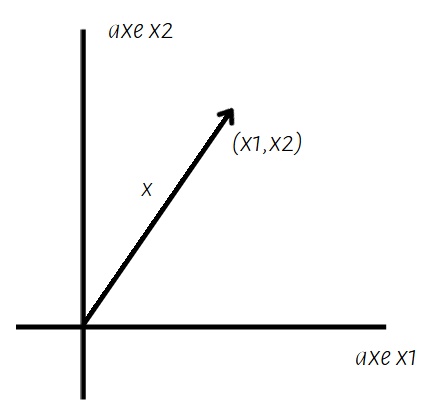
\includegraphics[scale=.45]{Chap1/vector1.png}\\
    \textit{Les éléments de $\R^2$ peuvent être vus comme des point ou des vecteurs.}
\end{center}
\noindent
Les axes et coordonnées explicites remplissent inutilement l'image ci-dessus, et on comprend souvent mieux en les supprimant et en pensant juste au vecteur, comme dans l'image ci-dessous.\\

\begin{center}
    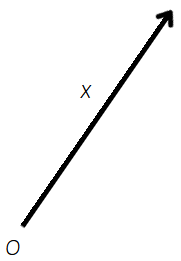
\includegraphics[scale=.45]{Chap1/vector2.png}\\
    \textit{Un vecteur}
\end{center}


Lorsque l'on utilise des images dans $\R^2$ ou le langage quelques peu vague des points et vecteurs, il faut se souvenir que ce ne sont que des aides à notre compréhension, et non pas des substituts pour les mathématiques effectives que nous allons développer. Même si nous ne pouvons dessiner de bonnes images dans des espaces à plus de dimensions, les éléments de ces dimensions sont définis aussi rigoureusement que ceux de $\R^2$. Par exemple, $(2,-3,17,\pi,\sqrt{2})$ est un élément de $\R^5$, et nous pouvons simplement nous référer à lui comme à un point ou un vecteur de $\R^5$ sans avoir à s'inquiéter de si la géométrie de $\R^5$ a le moindre sens physique.\\

\indent\marginpar{\flushleft{\textit{Les modèles mathématiques pour l'économie ont souvent des milliers de variables, par exemple $x_1,\ldots,x_{5000}$, ce qui veut dire que nous devons opérer dans $\R^{5000}$. Un tel espace ne peux pas être étudié géométriquement, mais l'approche algébrique fonctionne bien. C'est pour quoi notre sujet s'appelle l'\textbf{algèbre} linéaire.}}}
Souvenez-vous que nous définissons la somme de 2 éléments de $\K^n$ comme étant l'élément de $\K^n$ obtenue en additionnant les coordonnées correspondantes; comme vu en 0.0.1. Dans le cas particulier de $\R^2$, l'addition a une interprétation géométrique simple. Supposons que nous avons 2 vecteurs $x$ et $y$ dans $\R^2$ et que nous voulons les additionner, comme dans le côté gauche de l'image ci-dessous. Nous déplaçons le vecteur $y$ parallèle à lui-même pour que son origine coïncide avec l'extrémité de $x$. La somme $x+y$ est alors égale au vecteur dont l'origine correspond à celle de $x$ et l'extrémité à celle du nouveau vecteur $y$, comme sur le côté droit de l'image ci-dessous.\\

 

\begin{center}
    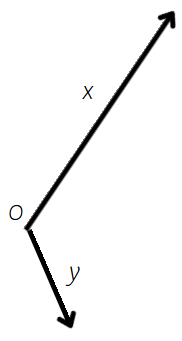
\includegraphics[scale=.45]{Chap1/2vectors.png}
    \hspace{1cm}
    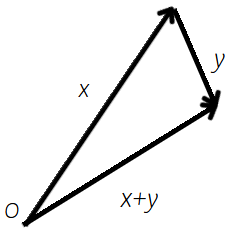
\includegraphics[scale=.45]{Chap1/2vectors2.png}\\
    \textit{La somme de 2 vecteurs}
\end{center}

Notre traitement du vecteur $y$ dans l'image ci-dessus illustre une philosophie standard lorsque nous pensons les vecteurs de $\R^2$ comme des flèches : nous pouvons les déplacer parallèles à elles-mêmes (sans changer leur longueur ou direction) et toujours avoir le même vecteur.\\
\indent
Maintenant que nous avons vu l'addition dans $\K^n$, nous nous tournons vers la multiplications. Nous pourrions définir la multiplication de manière similaire, en commançant avec 2 éléments de $\K^n$ et en en obtenant un nouveau en multipliant les coordonnées correspondantes. Cependant l'expérience nous montre que cette définition ne nous est pas utile. Un autre type de multiplication, appelé multiplication scalaire, sera centrale dans notre sujet. Spécifiquement, nous avons besoin de définir ce que veut dire multiplier un élément de $\K^n$ par un élément de $\K$. Nous choisissons la définition évidente : effectuer une multiplication sur chaque coordonné :
\begin{equation*}
    a(x_1,\ldots,x_n)=(ax_1,\ldots,ax_n)~;
\end{equation*}
ici $a\in\K$ et $(x_1,\ldots,x_n)\in\K^n$.\\
\indent
La multiplication scalaire a une belle interprétation géométrique dans $\R^2$. Si $a$ est un nombre positif et $x$ un vecteur de $\R^2$, alors $ax$ est le vecteur qui pointe dans la même direction que x et dont la longueur est $a$ fois celle de $x$. Autrement dit, pour obtenir $ax$, on rétrécit ou étire $x$ par un facteur $a$, en fonction de si $a<1$ ou $a>1$. La prochaine image illustre ceci.

\begin{center}
    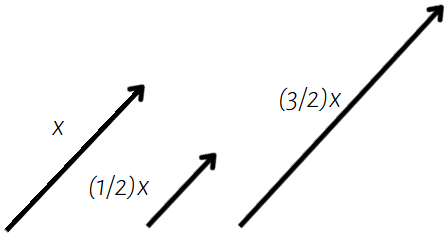
\includegraphics[scale=.45]{Chap1/PosMult.png}\\
    \textit{Multiplication par un scalaire positif}
\end{center}

\noindent
Si $a$ est un nombre négatif et $x$ un vecteur de $\R^2$, alors $ax$ est le vecteur qui pointe dans la direction opposée à $x$ et dont la longueur est $|a|$ fois la longueur de $x$, comme montré ci-dessous.

\begin{center}
    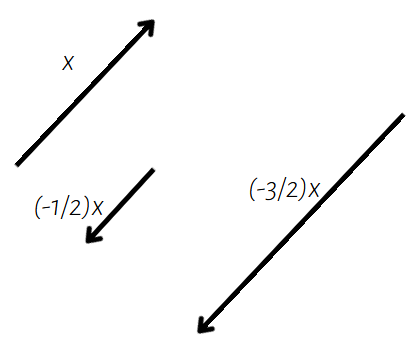
\includegraphics[scale=.45]{Chap1/NegMult.png}\\
    \textit{Multiplication par un scalaire négatif}
\end{center}

La motivation pour avoir défini un espace vectoriel vient des propriétés importantes de l'addition et de la multiplication scalaire de $\K^n$. En particulier, l'addition dans $\K^n$ est commutative et associative et possède un élément neutre, à savoir 0. Tout élément possède un opposé. La multiplication scalaire dans $\K^n$ est associative, et la multiplication scalaire par 1 fonctionne comme l’élément neutre. Enfin, l'addition et la multiplication dans $\K^n$ sont connectées par la distributivité.\\
\indent
Nous allons définir un espace vectoriel comme étant un ensemble $E$ ainsi qu'une addition et une multiplication scalaire dans $E$ qui satisfassent les propriétés énoncées dans le paragraphe précédent. Par une \textit{addition} sur $E$, nous voulons parler d'une fonction qui, à chaque paire d'éléments $u,v\in E$, assigne un élément $u+v$ dans $E$. Par une \textit{multiplication scalaire} dans $E$, nous voulons parler d'une fonction qui, à chaque $a\in\K$ et chaque $v\in E$, assigne un élément $av$ dans $E$.\\
\indent
Nous sommes désormais prêts pour donner une définition formelle d'un espace vectoriel. Un \textit{espace vectoriel} est un ensemble $E$ ainsi qu'une addition sur $E$ et qu'une multiplication scalaire sur $E$, tels que les propriétés suivantes s'appliquent :\\

\noindent
\textbf{Commutativité}\\
\indent{$u+v=v+u$ pour tous $u,v\in E$} ;\\

\noindent
\textbf{Associativité}\\
\indent{$(u+v)+w=u+(v+w)$ et $(ab)v=a(bv)$ pour tous $u,v,w\in E$ et tous\\
\indent $a,b\in\K$} ;\\

\noindent
\textbf{Élément neutre additif}\\
\indent{il existe un élément $0\in E$ tel que $v+0=v$ pour tout $v\in E$} ;\\

\noindent
\textbf{Opposé}\\
\indent{pour tout $v\in E$, il existe $w\in E$ tel que $v+w=0$} ;\\

\noindent
\textbf{Élément neutre multiplicatif}\\
\indent{$1v=v$ pour tout $v\in E$} ;\\

\noindent
\textbf{Distributivité}\\
\indent{$a(u+v)=au+av$ et $(a+b)v=av+bv$ pour tous $a,b\in\K$ et tous $u,v\in E$}.\\

\indent
La multiplication scalaire dans un espace vectoriel dépend de $\K$. De ce fait, si nous avons besoin d’être précis, nous dirons que $E$ est un espace vectoriel sur $\K$ au lieu de simplement dire que $E$ est un espace vectoriel. Par exemple, $\R^n$ est un espace vectoriel sur $\R$ et $\C^n$ est un espace vectoriel sur $\C$. Fréquemment, un espace vectoriel sur $\R$ est appelé un \textit{espace vectoriel réel} et un espace vectoriel sur $\C$ est appelé un \textit{espace vectoriel complexe}. Normalement, le choix de $\K$ est soit évident grâce au contexte, soit non pertinent, c'est pourquoi nous supposons souvent que $\K$ se cache en arrière-plan sans le mentionner spécifiquement.\\
\indent
Les éléments d'un espace vectoriel sont appelés \textit{vecteurs} ou \textit{points}. Ce langage géométrique aide parfois notre intuition.\\
\indent
Sans surprise, $\K^n$ est un espace vectoriel sur $\K$, comme vous devriez le vérifier. Naturellement, cet exemple a motivé notre définition d'espace vectoriel.\\
\indent\marginpar{\flushright{\textit{L'espace vectoriel le plus simple contient seulement 1 point. Autrement dit, \{0\} est un espace vectoriel, quoique très peu intéressant.}}}
Pour un autre exemple, considérez $\K^{\infty}$, qui est défini comme l'ensemble de toutes les séquences déléments de $\K$ :
\begin{equation*}
    \K^{\infty} = \{(x_1,x_2,\ldots):x_j\in\K \textrm{~pour~} j=1,2,\ldots\}.
\end{equation*}
L'addition et la multiplication scalaire sont définies sur $\K^{\infty}$ comme attendu :


%\begin{eqnarray*}
%        (x_1,x_2,\ldots)+(y_1,y_2,\ldots)=(x_&+y_1,x-2+y_2,\ldots)\\
%        a(x_1,x_2,\ldots)=(ax_1,ax_2,\ldots)
%\end{eqnarray*}

% Correction  Ne pas utiliser eqnarray voir https://www.tug.org/pracjourn/2006-4/madsen/madsen.pdf
\begin{equation*}
    (x_1,x_2,\ldots)+(y_1,y_2,\ldots)=(x_1+y_1,x-2+y_2,\ldots),
\end{equation*}
\begin{equation*}
    a(x_1,x_2,\ldots)=(ax_1,ax_2,\ldots).
\end{equation*}

Avec\marginpar{\flushright{\textit{Même si $\K^n$ est un exemple crucial d’espace vectoriel, tous les espaces vectoriels ne consistent pas de tuples. Par exemple, les éléments de $\mathcal{P}(\K)$ sont des fonctions sur $\K$ et non des tuples. En général. un espace vectoriel est une entité abstraite dont les éléments peuvent être des tuples, des fonctions, ou des objets étranges.}}} ces définitions, $\K^{\infty}$ devient un espace vectoriel sur $\K$, comme vous devriez le vérifier. L’élément neutre pour l'addition dans cet espace vectoriel est la séquence constituée uniquement de 0.\\
\indent
Notre prochain exemple est un espace vectoriel incluant des polynômes. Une fonction $p:\K\mapsto\K$ est appelée un \textit{polynôme} à coefficients dans $\K$ si il existe $a_0,\ldots,a_m\in\K$ tel que
\begin{equation*}
    p(z)=a_0+a_1z+a_2z^2+\ldots+a_mz^m
\end{equation*}
pour tout $z\in\K$. On définit $\mathcal{P}(\K)$ comme l’ensemble de tous les polynômes  à coefficients dans $\K$. L’addition dans $\mathcal{P}(\K)$ est définie comme vous vous y attendriez : si $p,q\in\mathcal{P}(\K)$, alors $p+q$ est le polynôme défini par
\begin{equation*}
    (p+q)(z)=p(z)+q(z)
\end{equation*}
pour $z\in\K$. Par exemple, si $p$ est le polynôme défini par $p(z)=2z+z^3$ et $q$ le polynôme défini par $q(z)=7+4z$, alors $p+q$ est le polynôme défini par $(p+q)(z)=7+6z+z^3$. La multiplication scalaire sur $\mathcal{P}(\K)$ a également une définition évidente : si $a\in\K$ et $p\in\mathcal{P}(\K)$, alors $ap$ est le polynôme défini par
\begin{equation*}
    (ap)(z)=ap(z)
\end{equation*}
pour $z\in\K$. Avec ces définitions de l’addition et de la multiplications scalaire, $\mathcal{P}(\K)$ est un espace vectoriel, comme vous devriez le vérifier. L’élément neutre additif dans cet espace vectoriel est le polynôme dont tous les coefficients sont égaux à 0.\\
\indent
Bientôt nous verrons d’autres exemples d’espace vectoriel, mais nous devons d’abord développer certaines des propriétés élémentaires des espaces vectoriels.\\


\section*{Propriétés des espaces vectoriels}

La définition d'un espace vectoriel requiert que ce dernier ait un élément neutre additif. La proposition ci-dessous énonce que cet élément est unique.\\

\begin{prop}
    Un espace vectoriel a un élément neutre additif unique.
    \begin{proof}
        Supposons que 0 et 0' sont tous deux des élément neutres d'un espace vectoriel $E$. Alors 
        \begin{equation*}
            0'=0'+0=0,
        \end{equation*}
        où la première équation vient du fait que 0 est un élément neutre, et la deuxième parce que 0' est aussi un élément neutre. Ainsi, $0=0'$, ce qui montre que $E$ ne possède qu'un seul élément neutre additif.\marginpar{\flushleft{\textit{Le symbole $\blacksquare$ signifie <<fin de la preuve>>.}}}
    \end{proof}
\end{prop}

Chaque élément $v$ d'un espace vectoriel a un opposé, un élément $w$ dans l'espace vectoriel teel que $v+w=0$. La proposition ci-dessous énonce que chaque élément dans un espace vectoriel a un unique opposé.\\

\begin{prop}
    Chaque élément dans un espace vectoriel a un unique opposé.
    \begin{proof}
        Supposons que $E$ est un espace vectoriel avec $v\in E$. Supposons que $u$ et $w$ sont des opposés de $v$. Alors
        \begin{equation*}
            u=u+0=u+(v+w)=(u+v)+w=0+w=w.
        \end{equation*}
        Ainsi, $u=w$ comme désiré.
    \end{proof}
\end{prop}

Maintenant que nous savons que l'opposé est unique, pour $v$ un élément d'un espace vectoriel, on peut noter $-v$ l'opposé de $v$. On définit $w-v$ comme signifiant $w+(-v)$.\\
\indent
Presque tous les résultats de ce livre vont inclure des espaces vectoriels. Pour éviter d'être distrait par le fait d'avoir à redire sans arrêt une phrase comme <<Supposons que $E$ est un espace vectoriel>>, nous allons maintenant faire la déclaration nécessaire une fois pour toutes :

\begin{center}
    \begin{tabular}{|c|}
        \hline
        Mettons-nous d'accord que pour le reste du livre,   \\
        $E$ désignera un espace vectoriel sur $\K$.   \\
        \hline
    \end{tabular}
\end{center}

Grâce à l'associativité, nous pouvons oublier les parenthèses lorsque nous manipulons des additions à plus de 2 éléments dans un espace vectoriel. Par exemple, nous pouvons écrire $u+v+w$ sans parenthèses puisque les 2 interprétations possibles de cette expressions, à savoir $(u+v)+w$ et $u+(v+w)$, sont égales. Nous utliserons cette conventions familière de ne pas utiliser de parenthèses dans la prochaine preuve. Dans la prochaine proposition, 0 désigne un scalaire (le nombre $0\in\K$) du côté gauche de l'équation et un vecteur (l'élément neutre additif de $E$) du côté droit de l'équation.\\

\marginpar{\flushright{\textit{Notez que 1.4 et 1.5 parlent de la multiplication scalaire et de l'élément neutre additif de $E$. La seule partie de la définition d'un espace vectoriel qui relie la multiplication scalaire et l'addition de vecteurs est la distributivité. De ce fait, la distributivité doit être utilisée dans les preuves.}}}
\begin{prop}
    $0v=0$ pour tout $v\in E$.
    \begin{proof}
        Pour $v\in E$, nous avons
        \begin{equation*}
            0v=0v+0v-0v=(0+0)v-0v=0v-0v=0,
        \end{equation*}
        comme voulu.
    \end{proof}
\end{prop}

Dans la prochaine proposition, 0 désignera l'élément neutre additif de $E$. Même si leur preuves sont similaires, 1.4 et 1.5 ne sont pas identiques. Plus précisément, 1.4 dit que le produit du scalaire 0 avec n'importe quel vecteur est égal au vecteur 0, tandis que 1.5 dit que le produit de n'importe quel scalaire avec le vecteur 0 donne le vecteur 0.\\

\begin{prop}
    $a0=0$ pour tout $a\in\K$.
    \begin{proof}
        Pour $a\in\K$, on a
        \begin{equation*}
            a0=a0+a0-a0=a(0+0)-a0=a0-a0=0,
        \end{equation*}
        comme voulu.
    \end{proof}
\end{prop}

Maintenant nous allons montrer que si un élément de $E$ est multiplié par le scalaire $-1$, alors le résultat est l'opposé de l'élément de $E$.

\begin{prop}
    $(-1)v=-v$ pour tout $v\in E$.
    \begin{proof}
        Pour $v\in E$, on a
        \begin{equation*}
            v+(-1)v=1v+(-1)v=(1+(-1))v=0v=0,
        \end{equation*}
        Cette équation dit que $(-1)v$, quand il est additionné à $v$, donne 0. De ce fait, $(-1)v$ doit être l'opposé de $v$, comme voulu.
    \end{proof}
\end{prop}

\section*{Sous-espaces vectoriels}

Un {\marginpar{\flushleft{\textit{Certains mathématiciens utilisent le terme \textbf{sous-espace linéaire}, ce qui veut dire la même chose que sous-espace vectoriel}}}} sous-ensemble $F$ de $E$ est appelé \textit{sous-espace vectoriel} de $E$ si $F$ est également un espace vectoriel (en utilisant les mêmes addition et multiplication scalaire que dans $E$). Par exemple,
\begin{equation*}
    \{(x_1,x_2,0):x_1,x_2\in\K\}
\end{equation*}
est un sous-espace vectoriel de $\K^3$. Si $F$ est un sous-ensemble de $E$ non vide, alors pour vérifier que $F$ est un sous-espace vectoriel de $E$, nous avons seulement besoin de vérifier que $F$ satisfait les propriétés suivantes :\\

\noindent
\textbf{Stabilité pour l'addition}\\
\indent{$u,v\in F$ implique que $u+v\in F$}\\

\noindent
\textbf{Stabilité pour la multiplication scalaire}\\
\indent{$a\in\K$ et $u\in F$ implique que $au\in F$}\\

\noindent
La première condition {\marginpar{\flushleft{\textit{Il est évident que \{0\} est le plus petit sous-espace vectoriel de $E$ et que $E$ lui-même est le plus grand. L'ensemble nul n'est pas un sous-espace vectoriel de $E$ parce qu'un sous-espace vectoriel doit être un espace vectoriel et qu'un espace vectoriel doit contenir au moins un élément, à savoir un élément neutre additif.}}}}, qui peut être décrite en disant que $F$ est \textit{fermé sous l'addition}, assure que l'addition a un sens dans $F$. La seconde, qui peut être décrite en disant que $F$ est \textit{fermé sous la multiplication scalaire}, assure que la multiplication scalaire a un sens dans $F$. Pour montrer que $F$ est un espace vectoriel, les autres parties de la définition d'un espace vectoriel n'ont pas besoin d’être vérifiées, car elles sont automatiquement satisfaites. Par exemple, l'associativité et la commutativité de l'addition sont automatiquement valables dans $F$ car elles le sont dans le plus grand espace $F$. Pour donner un autre exemple, si la seconde condition ci-dessus est vraie et que $u\in F$, alors $-u$ (qui est égal à $(-1)u$ par 1.6), est également dans $F$, et de ce fait tout élément de U a un opposé dans $F$.\\
\indent
Les 2 conditions ci-dessus nous permettent généralement de déterminer rapidement si un sous-ensemble de $E$ donné est ou non un sous-espace vectoriel de $E$. Par exemple, si $b\in\K$, alors
\begin{equation*}
    \{(x_1,x_2,x_3,x_4)\in\K^4:x_3=x_4+b\}
\end{equation*}
est un sous-espace vectoriel de $\K^4$ si, et seulement si $b=0$, comme vous devriez le démontrer. Pour un autre exemple, vous devriez démontrer que
\begin{equation*}
    \{p\in \mathcal{P}(\K):p(3)=0\}
\end{equation*}
est un sous-espace vectoriel de $\mathcal{P}(\K)$.\\
\indent
Les sous-espaces vectoriels de $\R^2$ sont précisément \{0\}, $\R^2$, et toutes les lignes de $\R^2$ passant par l'origine. Les sous-espaces vectoriels de $\R^3$ sont précisément \{0\}, $\R^3$, toutes les lignes de $\R^3$ passant par l'origine, et tous les plans de $\R^3$ passant par l'origine. Prouver que tous ces objets sont en effet des sous-espaces vectoriels est simple---la partie compliquée est de montrer que ce sont les seuls sous-espaces vectoriels de $\R^2$ ou de $\R^3$. Cette tâche sera plus simple après avoir introduit quelques outils supplémentaires dans le chapitre suivant.

\section*{Sommes et sommes directes}
Dans des chapitres futurs, nous trouverons que les notions de somme et somme directe d'espace vectoriel sont utiles. Nous allons donc ici définir ces concepts.\\
\indent
Supposons que $F_1,\ldots,F_m$ sont des sous-espaces vectoriels de $E$. La \textit{somme} de $F_1,\ldots,F_m$, notée $F_1+\ldots+F_m$, est définie comme l'ensemble de toutes les sommes possibles d'éléments de $F_1,\ldots,F_m$. Plus précisément,
\begin{equation*}
    F_1+\ldots+F_m=\{u_1+\ldots+u_m:u_1\in F_1,\ldots,u_m\in F_m\}
\end{equation*}

Vous devriez vérifier que si $F_1,\ldots,F_m$ sont des sous-espaces vectoriels de $E$, alors la somme $F_1+\ldots+F_m$ est un sous-espace vectoriel de $E$. \marginpar{\flushleft{\textit{Lorsque l'on manipule des espaces vectoriels, nous sommes généralement seulement intéressés par les sous-espaces vectoriels, et non pas par des sous-ensembles arbitraires. L'union d'espace vectoriels est rarement un espace vectoriel (voir l'exercice 9 de ce chapitre), c'est pourquoi nous travaillons surtout avec des sommes plutôt que des unions.}}}\\

Regardons quelques exemples de somme de sous-espaces vectoriels. Supposons que $F$ est l'ensemble de tous les éléments de $\K^3$ dont la deuxième et troisième coordonnée est égale à 0, et que $E$ est l'ensemble de tous les éléments de $\K^3$ dont la première et troisième coordonnée est égale à 0 :
\begin{equation*}
    F=\{(x,0,0)\K^3:x\in\K\} \textrm{~et~} G=\{(0,y,0)\K^3:y\in\K\}
\end{equation*}
Alors
\begin{prop}
    \begin{equation*}
        F+G=\{(x,y,0):x,y\in\K\}
    \end{equation*}
\end{prop}
comme vous devriez le vérifier.\\
\indent
Pour un autre exemple, supposez que $F$ est défini comme ci-dessus, et que $G$ est l'ensemble de tous les élément de $\K^3$ dont la première et la deuxième coordonnée sont égales, et la troisième vaut 0 :
\begin{equation*}
    G=\{(y,y,0)\K^3:y\in\K\}
\end{equation*}
Alors $F+G$ est aussi donné par 1.7, comme vous devriez le vérifier.\\

\indent
\marginpar{\flushright{\textit{Les sommes d'espaces vectoriels en théorie des espaces vectoriels sont analogues aux unions d'ensembles en théorie des ensemble. Si on a 2 sous-espaces vectoriels d'un espace vectoriel, le plus petit sous-espace vectoriel contenant les 2 premiers est leur somme. Analoguement, si on a 2 sous-ensemble d'un ensemble, le plus petit sous-ensemble les contenant est leur somme.}}}Supposons que $F_1,\ldots,F_m$ sont des sous-espaces vectoriels de $E$. évidemment, $F_1,\ldots,F_m$ sont tous contenus dans $F_1+\ldots+F_m$ (pour voir cela, considérez la somme $u_1+\ldots+u_m$ où tous les $u$ sauf 1 valent 0). à l'inverse, tout sous-espace vectoriel de $E$ contenant $F_1,\ldots,F_m$ doit contenir $F_1+\ldots+F_m$ (puisqu'un sous-espace vectoriel doit contenir toutes les sommes finies de ses éléments). De ce fait, $F_1+\ldots+F_m$ est le plus petit sous-espace vectoriel de $V$ contenant $F_1,\ldots,F_m$.\\

Supposons que $F_1,\ldots,F_m$ sont des sous-espaces vectoriels de $E$ tels que $E=F_1+\ldots+F_m$. De ce fait, tout élément de $E$ peut être écrit sous la forme
\begin{equation*}
    u_1+\ldots+u_m
\end{equation*}
où chaque $u_j\in F_j$. Nous serons en particulier intéressés par les cas où chaque vecteur de $F$ peut être représenté de manière unique sous la forme ci-dessus. Cette situation est tellement importante que nous lui donnons un nom particulier : une somme directe. En particulier, nous disons que $F$ est la \textit{somme directe} des sous-espaces vectoriels $F_1,\ldots,F_m$, écrit $E=F_1\oplus\ldots\oplus F_m$, si chaque élément de $V$ peut être écrit de manière unique comme une somme $u_1+\ldots+u_m$ où chaque $u_j\in F_j$.\\

Regardons quelques exemples de somme directe. Supposons que $F$ est le sous-espace vectoriel de $\K^3$ constitué de ses vecteurs dont la dernière coordonnée vaut 0, et $G$ le sous-espace vectoriel de $\K^3$ constitué de ses vecteurs dont la première et deuxième coordonnée vaut 0 :
\begin{equation*}
    U=\{(x,y,0)\in\K^3:x,y\in\K\} \textrm{~et~} W=\{(0,0,z)\in\K^3:z\in\K\}
\end{equation*}
Alors $\K^3=F\oplus G$, comme vous devriez le vérifier.\\

Comme autre exemple, supposons que $F_j$ est le sous-espace vectoriel de $\K^n$ constitué de ses vecteurs dont toutes les coordonnées valent 0, exceptées possiblement en $j\ieme$ position (par exemple, $F_2=\{(0,x,0,\ldots,0)\in\K^n:x\in\K\}$). Alors on a
\begin{equation*}
    \K^n=F_1\oplus\ldots\oplus F_n
\end{equation*}
comme vous devriez le vérifier.\marginpar{\flushleft{\textit{Le symbole $\oplus$, constitué d'un signe plus à l'intérieur d'un cercle, est utilisé pour rappeler que nous travaillons avec un type particulier de somme de sous-espaces vectoriels---chaque élément dans une somme directe peut être représenté de manière unique comme une somme d'éléments des sous-espaces vectoriels sommés.}}}\\

Pour notre dernier exemple, considérons l'espace vectoriel $\mathcal{P}(\K)$ de tous les polynômes à coefficient dans $\K$. $F_p$ désigne le sous-espace vectoriel de $\mathcal{P}(\K)$ constitué de tous les polynômes $p$ de la forme
\begin{equation*}
    p(z)=a_0+a_2z^2+\ldots+a_{2m}z^{2m}
\end{equation*}
et $F_i$ désigne le sous-espace vectoriel de $\mathcal{P}(\K)$ constitué de tous les polynômes $p$ de la forme
\begin{equation*}
    p(z)=a_1z+a_3z^3+\ldots+a_{2m+1}z^{2m+1}
\end{equation*}
ici $m$ est un entier positif, et $a_0,\ldots,a_{2m+1}\in\K$ (les notations $F_p$ et $F_i$ devraient vous rappeler le puissances paires et impaires de $z$). Vous devriez vérifier que
\begin{equation*}
    \mathcal{P}(\K)=F_p\oplus F_i
\end{equation*}

Parfois un contre-exemple nous aide à comprendre autant qu'un exemple. Considérez les 3 sous-espaces vectoriels suivants de $\K^3$ :
\begin{eqnarray*}
    F_1=\{(x,y,0)\in\K^3:x,y\in\K\}\\
    F_2=\{(0,0,z)\in\K^3:z\in\K\}\\
    F_3=\{(0,y,y)\in\K^3:y\in\K\}\\
\end{eqnarray*}
Clairement $\K^3=F_1+F_2+F_3$ car un vecteur arbitraire $(x,y,z)\in\K^3$ peut être écrit sous la forme
\begin{equation*}
    (x,y,z)=(x,y,0)+(0,0,z)+(0,0,0)
\end{equation*}
où le premier vecteur du côté droit appartient à $F_1$, le deuxième à $F_2$ et le troisième à $F_3$. Cependant $\K^3$ n'est pas égal à la somme directe de $F_1,F_2,F_3$ car le vecteur $(0,0,0)$ peut être écrit de 2 façon différentes comme une somme $u_1+u_2+u_3$, avec chaque $u_j\in F_j$. Spécifiquement, on a
\begin{equation*}
    (0,0,0)=(0,1,0)+(0,0,1)+(0,-1,-1)
\end{equation*}
et, évidemment,
\begin{equation*}
    (0,0,0)=(0,0,0)+(0,0,0)+(0,0,0)
\end{equation*}
où le premier vecteur du côté droit de chaque équation appartient à $F_1$, le deuxième à $F_2$ et le troisième à $F_3$.\\
\indent
Dans l'exemple ci-dessus, on a montré que nous n'avions pas de somme directe en montrant que 0 n'avait pas de représentation unique comme une somme de vecteurs appropriés. La définition d'une somme directe requiert que chaque vecteur dans l'espace ait une unique représentation comme une somme appropriée. Supposons que nous ayons une collection de sous-espaces vectoriels dont la somme vaut l'espace vectoriel entier. La prochaine proposition montre que lorsque l'on cherche si cette collection de sous-espaces vectoriels est une somme directe, nous avons seulement besoin de vérifier si 0 peut être exprimé de manière unique.

\begin{prop}
    Supposons que $F_1,\ldots,F_n$ sont des sous-espaces vectoriels de $E$. Alors $E=F_1\oplus\ldots\oplus F_n$ si, et seulement si, les conditions suivantes sont respectées :
    \begin{description}
        \item[(a)] $ E=F_1+\ldots+F_n $
        \item[(b)] le seul moyen d'écrire 0 comme une somme $u_1+\ldots+u_n$ où chaque $u_j\in F_j$ est de prendre chaque $u_j$ égal à 0
    \end{description}
\end{prop}

\textsc{Preuve :} Supposons d'abord que $E=F_1\oplus\ldots\oplus F_n$. évidemment (a) est vérifié (cela vient de comme la somme et la somme directe sont définies). Pour prouver (b), supposons que $u_1\in F_1,\ldots,u_n\in F_n$ et
\begin{equation*}
    0=u_1+\ldots+u_n
\end{equation*}
Alors chaque $u_j$ doit valoir 0 (cela vient de l'unicité dans la définition de la somme directe, car $0=0+\ldots+0$ et $0\in F_1,\ldots,0\in F_n$), ce qui prouve (b).\\
\indent
Maintenant, supposons que (a) et (b) sont vrais. Soit $v\in E$. Par (a), nous pouvons écrire $v=u_1+\ldots+u_n$ avec $u_1\in F_1,\ldots,u_n\in F_n$. Pour montrer que cette représentation est unique, supposons que nous avons également $v=v_1+\ldots+v_n$ avec $v_1\in F_1,\ldots,v_n\in F_n$. En soustrayant les deux équations, on obtient
\begin{equation*}
    0=(u_1-v_1)+\ldots+(u_n-v_n)
\end{equation*}
\indent Clairement, $u_1-v_1\in F_1,\ldots,u_n-v_n\in F_n$, donc l'équation ci-dessus et (b) impliquent que chaque $u_j-v_j=0$. Ainsi, $u_1=v_1,\ldots,u_n=v_n$, comme voulu. \hfill$\blacksquare$

La prochaine proposition donne une condition simple pour tester quelles paires de sous-espaces vectoriels donne une somme directe. Notez que cette proposition traite seulement du cas avec 2 sous-espaces vectoriels. Lorsque vous vous demandez si la somme de plus de 2 sous-espaces vectoriels est directe, il n'est pas suffisant de tester si n'importe quelle paire de sous-espaces vectoriels s'intersectent seulement en 0. Pour voir cela, considérez le contre-exemple présenter juste avant 1.8. Dans ce contre-exemple nous avions $\K^3=F_1+F_2+F_3$, mais $\K^3$ n'étais pas égal à la somme directe de $F_1,F_2,F_3$. Cependant, dans ce contre-exemple, Nous avons $F_1 \cap F_2=F_2 \cap F_3=F_3 \cap F_1=\{0\}$ (comme vous devriez le vérifier). La prochaine proposition montre qu'avec seulement 2 sous-espaces vectoriels nous avons une condition nécessaire et suffisante pour qu'un somme soit directe.


\begin{prop}
    Supposons\marginpar{\flushleft{\textit{La somme de sous-espaces vectoriels est analogue à l'union de nous-ensembles. Similairement, la somme directe est analogue à l'union disjointe de sous-ensembles. Bien sûr, 2 sous-espaces vectoriels ne peuvent être disjoint, car ils doivent tous deux contenir 0. Donc la disjointness est remplacée, au moins pour le cas de 2 sous-espaces vectoriels, par la contrainte que l'intersection égale \{0\}.}}} que $F$ et $G$ soient des sous-espaces vectoriels de $E$. Alors $E=F\oplus G$ si, et seulement si, $E=F+G$ et $F \cap G=\{0\}$.
\end{prop}
\textsc{Preuve :} Supposons d'abord que $E=F\oplus G$. Alors $E=F+G$ (par la définition d'une somme directe). De plus, si $v\in F \cap G$, alors $0=v+(-v)$, où $v\in F$ et $-v\in F$. Par l'unicité de la représentation de 0 comme la somme d'un vecteur dans $F$ et d'un vecteur dans $G$, nous devons avoir $v=0$. De ce fait, $F\cap G=\{0\}$, ce qui finit la preuve dans un sens.\\
\indent
Pour prouver la proposition dans l'autre sens, supposons maintenant que $E=F+G$ et $F\cap G=\{0\}$. Pour prouver que $E=F\oplus G$, supposons que
\begin{equation*}
    0=u+w
\end{equation*}
où $u\in F$ et $w\in G$. Pour compléter la preuve, nous avons seulement besoin de montrer que $u=w=0$ (par 1.8). L'équation ci-dessus implique que $u=-w\in G$. Ainsi $u\in F\cap G$, et donc $u=0$. Ceci, accompagné de l'équation ci-dessus, implique que $w=0$, ce qui complète la preuve. \hfill$\blacksquare$.





% A ajouter vers la ligne 460 : \marginpar{\Klushleft{\textit{Le symbole $\oplus$, constitué d'un signe plus à l'intérieur d'un cercle, est utilisé pour rappeler que nous travaillons avec un type particulier de somme de sous-espaces vectoriels---chaque élément dans une somme directe peut être représenté de manière unique comme une somme d'éléments des sous-espaces vectoriels sommés.}}}%
\end{document}